\section{E-Mails und deren Tücken}
Täglich werden heute bis zu 180 Milliarden E-Mails versendet. Eine gewaltige Menge, wenn man bedenkt, dass es ein wenig mehr als sieben Milliarden Menschen auf diesem Planeten gibt.
Doch nur wenige E-Mail-Nutzer machen sich wohl Gedanken darüber, was denn eigentlich hinter einer E-Mail steckt. Wohin geht sie genau? Wer kann diese E-Mail theoretisch lesen? Wo wird diese Nachricht überall gespeichert? Und für wie lange? Gibt es Kopien? Backups? Auf anderen Servern?
All diese Fragen sind sehr wichtig, wenn man vertrauliche Daten per Mail versendet. Doch auch wenn der Inhalt der Nachricht nicht von grosser Bedeutung ist, möchte man eine gewisse Privatsphäre wahren, oder?
Was kann man also als „0815“ Nutzer tun, um seine eigenen E-Mails möglichst sicher zu versenden, zu speichern und zu empfangen?
\\
Im nächsten Kapitel wird versucht auf diese Fragen eine Antwort zu finden. Zuerst einmal muss man aber verstehen, wie das genau funktioniert mit den „Mails“.

\subsection{Funktionsweise des Mailverkehrs}

\begin{figure}[H]
\centering
\noindent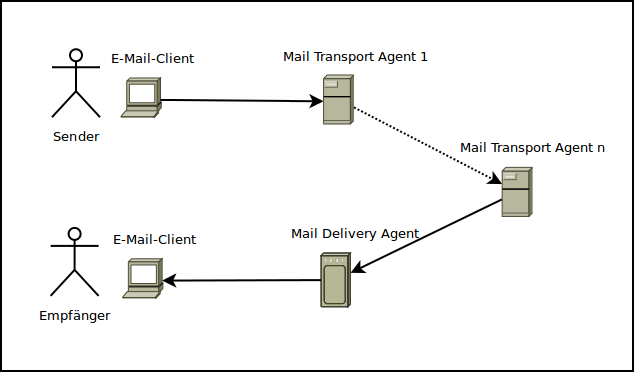
\includegraphics[scale=0.55]{images/email_function}
\caption{Funktionsweise des Mailverkehrs}
\end{figure}

Eine E-Mail passiert von der Erzeugung beim Sender bis zur Abgabe beim Empfänger mehrere Posten. Um die Funktionsweise des E-Mail-Verkehrs beschreiben zu können, müssen diese Posten zuerst erklärt werden:

\begin{itemize}
\item E-Mail-Client: Beim Client handelt es sich um das Mail-Programm, welches E-Mails senden und empfangen kann. Sowohl der Sender als auch der Empfänger sind auf ein solches angewiesen.
\item Mail Transfer Agent (MTA): Der Mail Transfer Agent ist für den Transport der E-Mail verantwortlich.
\footnote{Wikipedia: Mail Transport Agent, Linkverzeichnis, Link 16}
\item Mail Delivery Agent (MDA): Der Mail Delivery Agent hat die Aufgabe, die E-Mail beim Empfänger abzuliefern, sobald diese vom Mail Transfer Agent übermittelt wurde.
\footnote{Wikipedia: Mail Delivery Agent, Linkverzeichnis, Link 17}
\end{itemize}

Bei MTA und MDA handelt es sich jeweils um Computer-Programme, welche typischerweise auf den Servern (Computern) des jeweiligen Providers laufen.
\\
\\
Ablauf des E-Mail-Verkehrs:

\begin{enumerate}
\item Der Sender verfasst mit Hilfe des Clients eine Mail für einen bestimmten Empfänger und drückt anschliessend auf \textit{Senden}.
\item Der Client übermittelt die E-Mail bei aktiver Internetverbindung an den ersten MTA.
\item Die Mail wird nun von MTA zu MTA geschickt, bis derjenige des Empfängers gefunden wird.
\item Der MTA des Empfängers übermittelt die Mail an den MDA, welcher die Mail aufbewahrt.
\item Der Client des Empfängers holt die Mail bei aktiver Internetverbindung beim MDA ab und stellt sie dem Empfänger zur Verfügung.
\end{enumerate}

Je nach verwendetem Protokoll wird dem Empfänger eine Kopie der Mail zugestellt (IMAP), wobei das Original auf dem Server bleibt, oder er erhält das Original selbst (POP3).
\\
\\
IMAP (Internet Message Access Protocol) hat den Vorteil, dass man im Falle eines lokalen Datenverlusts das Original des Mails auf dem Server hat. Es eignet sich zudem sehr gut für die parallele Nutzung von mehreren Geräten (Computer, Tablet, Smartphone), da die E-Mails jeweils synchronisiert (abgeglichen) werden.
\footnote{Wikipedia: POP3, Linkverzeichnis, Link 18}
\\
\\
POP3 (Post Office Protocol 3) bietet diese Möglichkeiten nicht. Es eignet sich aber für Nutzer, die gerne selbst bestimmen, wo ihre E-Mails aufbewahrt werden. Seit den Snowden-Enthüllungen scheint dieses Argument wichtiger denn je.
\footnote{Wikipedia: IMAP, Linkverzeichnis, Link 19}

\subsection{Mein Provider und seine Server}
Der erste Schritt, den man tun muss, um überhaupt eine E-Mail versenden zu können, ist es, sich einen passenden Provider auszusuchen. Ein Provider ist eine Firma, die ihren Kunden eine Mail-Adresse zur Verfügung stellt. Dies kann z.B. Google mit Gmail, Microsoft mit Hotmail oder eine Firma wie GMX sein. Der Provider muss diese E-Mail-Adresse konfigurieren, damit der Kunde sie gebrauchen kann. Zur Konfiguration gehört unter anderem die Adresse zum Mail Transfer Agent und die Adresse zum Mail Delivery Agent.
Diese Programme bzw. die Server, auf denen sie laufen, sind nicht nur in Bezug auf die allgemeine Mailfunktionalität von Bedeutung. Nein, denn dort, auf diesen Servern, unter der Kontrolle des jeweiligen Providers, geht jede einzelne E-Mail, die versendet oder empfangen wird, durch. Das bedeutet, dass dort theoretisch ein Mitschnitt aller Nachrichten gemacht werden kann. Auch macht der Provider, natürlich nur zum Besten seiner Kunden, Backups (Sicherungen) von deren Postfächer. Das mag ja schön und gut sein und ist im Falle eines Datenverlusts äusserst praktsich, aber wer kann sonst noch auf dieses Postfach oder die Backup-Daten zugreifen? Die Systemadministratoren vom Provider? PR-Firmen? Datenanalysten? Geheimdienste? Wer weiss.

\subsection{E-Mails verschlüsseln}
Doch es gibt ein paar Dinge, die man tun kann, um seine E-Mails besser vor ungewollten Blicken zu schützen.
So gibt es mehrere Verfahren, um E-Mails zu verschlüsseln. Eines der beliebtesten und wohl meist verbreitetsten hierfür ist PGP (Pretty Good Privacy) oder deren Weiterentwicklung GPG (GNU Privacy Guard).
Bei beiden handelt es sich um ein Public-Key-Verfahren mit asymmetrischer Verschlüsselung. Bei dieser Art von Verschlüsselung gibt es einen öffentlichen Schlüssel, mit dem jeder Sender Daten für den Empfänger verschlüsseln und signieren kann und es gibt einen privaten, geheimen Schlüssel, der vom Empfänger benutzt wird, um die Nachricht, die mit seinem öffentlichen Schlüssel verschlüsselt wurde, wieder zu entschlüsseln.
Solange man seinen privaten Schlüssel geheim hält, ist es für einen ``Angreifer'' sehr schwierig sowie rechen- und zeitintensiv eine solche verschlüsselte Nachricht zu knacken.
Es gibt eine Menge Erweiterungen für die gängigsten Mail-Clients, um diese Verschlüsselungsfunktion nachzurüsten. Im Internet findet man viele Anleitungen, die einem zeigen, wie man dazu vorgehen muss und welche Erweiterungen sich empfehlen.

\subsection{Ich als Provider}
Wenn man plant, seine Mails selbst zu verwalten und komplett auf einen Mail-Provider zu verzichten, muss man sich fragen, was einen Provider ausmacht und welche Aufgaben er hat.
\\
Ein Provider muss einen MDA und einen MTA zur Verfügung stellen, damit Mails versendet und empfangen werden können. Diese müssen am Internet angehängt sein und dauerhaft laufen, damit die E-Mails ihr Ziel auch erreichen.
\\
Ausserdem muss er die E-Mail-Adresse des Kunden so konfigurieren, dass die Mails den richtigen Weg nehmen. Jeder Provider hat seine eigene Domain, wie zum Beispiel Google's \textit{gmail.com} oder Swisscom's \textit{bluewin.ch}. Die E-Mail-Adressen der Kunden enden deshalb immer auf jene Domains: \textit{max@gmail.com}, \textit{muster@bluewin.ch}. Als ``Selbstversorger'' braucht man nun ebenfalls eine solche Domain. Dabei muss es sich nicht zwingend um eine Top-Level-Domain handeln \footnote{Wikipedia: Top Level Domain, Linkverzeichnis, Link 20}. Auch eine kostenlose Domain mit der Endung \textit{.ch.vu} würde genügen.
\\
Dieser Domain braucht man dann nur noch einen DNS-Server \footnote{Wikipedia: Domain Name System, Linkverzeichnis, Link 21} zuzuweisen, der den MDA kennt.
Ein Problem gibt es da aber noch. Normale Haushaulte bekommen vom Internetprovider standardmässig keine statische IP-Adresse zugewiesen, was bedeutet, dass diese ständig ändern kann und so der DNS-Server nicht mehr weiss, wohin er jetzt den Datenverkehr weiterleiten muss. Um dieses Problem zu lösen gibt es zwei Möglichkeiten: Man kann beim Provider eine kostenpflichtige statische IP-Adresse erwerben oder man registriert sich bei einem dynamischen DNS-Anbieter. Dieser stellt eine Schnittstelle zur Verfügung, über die man die IP-Adresse seines Server bei jeder Änderung dem DNS-Server mitteilen kann. Somit kennt der DNS-Server stets die aktuelle IP-Adresse des Servers.
\\
\\
\textit{Hinweis: IP-Adressen und DNS-Server werden in Kapitel 6 - Surfen im Internet noch genauer erklärt.}

\subsubsection{Vor- und Nachteile}
Natürlich gibt es nicht nur Vorteile, wenn man sein eigener E-Mail-Provider ist. Eine kurze Auflistung einiger Vor- und Nachteile soll eine Übersicht bieten.
\\

\textbf{Vorteile:}
\begin{itemize}
    \item Volle Kontrolle
    \item Verschlüsselung
    \item Eigener Spam und Virenfilter
\end{itemize}

\textbf{Nachteile:}
\begin{itemize}
    \item Hardware- und Unterhaltungs-Kosten
    \item Benötigte Zeit bzw. benötigtes Know-How
    \item Risiko von Datenverlust
\end{itemize}

\subsection{Vertrauenswürdige Provider?}
Seine Mails selbst zu verwalten ist ein schwieriges unterfangen und mit viel Aufwand verbunden. Für Laien ist dies definitiv keine empfehlenswerte Lösung. Die Frage, die sich deshalb stellt ist, ob es denn bereits vertrauenswürdige und sichere E-Mail Provider gibt, auf die man stattdessen zurückgreifen kann. \\
Leider ist es sehr schwierig oder gar unmöglich eine Antwort auf diese Frage zu finden, denn Tatsache ist, dass in der Theorie jeder Provider gehackt werden kann. Die Daten sind beim Provider somit nie hundert Prozent sicher. \\
Es bleibt einem nichts anderes übrig, als zu vertrauen. Vertrauen in den Provider, dass dieser bestrebt ist, jede mögliche Massnahme zu treffen, um die höchsten Sicherheitsstandards einzuhalten. \\
Ein Beispiel hierfür ist \textit{NEOMAILBOX}\footnote{Neomailbox, Linkverzeichnis, Link 21}. Diese Firma stellt einen kostenpflichtigen Service zur Verfügung, der einen schnellen, sicheren und anonymen E-Mail-Dienst verspricht. Zudem soll der Service mit einem top Spam- und Virenfilter ausgestattet sein.\footnote{Neomailbox, Linkverzeichnis, Link 22}
